\section{Data} \label{data_lab}
In Chapter \ref{cont_vol} wee looked into the assumption of constant volatility in the Black Scholes model. 
Where during the study, a 10Y10Y EUR swaption was introduced. This chapter will provide a introduction to 
market data on swaptions. In this thesis the data source is Citi Velocity, which is a market data plantformed
owned by Citi Bank.
\\\\
Before delving into the market data on swaptions, let's revisit the definition of a swaption. 
A swaption gives the holder the right, but not the obligation, to enter into an interest rate swap in the future. 
There are two types of swaptions: payer swaptions and receiver swaptions, as previously described.
\\\\
The four main parameters defining a swaption are:
\begin{itemize}
\item \textbf{Expiry} \text{---}  when in the future the holder can exercise their right.
\item \textbf{Tenor} \text{---}  the maturity of the underlying interest rate swap.
\item \textbf{Strike} \text{---}  the pre-specified interest rate of the swap.
\item \textbf{Pay/Receive} \text{---}  whether the holder pays or receives the fixed rate.
\end{itemize}
\noindent
As mentioned a 10Y10Y EUR swaption was analyzed, but let's clarify what a 10Y10Y EUR swaption entails. 
Assuming the swaption is a receiver swaption, it represents a contract that, in ten years, 
gives the holder the right to enter into a ten year interest rate swap in EUR, receiving a fixed rate. 
Thus, the swaption has an expiry of 10 years, a tenor of 10 years, and a strike equivalent to the value of the fixed rate. 
It is important to note that the underlying interest rate swap in the swaption is a forward swap, commencing 10 years from now: 
the settlement date.
\\\\
Then before we will look at some displayed data, let's first cover some lingo of swaption. 
A swaption with a strike set at the current market rate for the underlying forward swap is referred 
to as at-the-money-forward (ATMF). If the strike differs from the ATMF rate, the swaption is categorized as out-of-the-money (OTM).
\\\\
When discussing swaptions, it is essential to recognize how the volatility surface or smile varies across different expiries and swap 
forward tenors. Displayed below in \autoref{tab:swaption_skew_ATMF} is the ATMF swaption volatility surface. 
The presentation of the volatility surface in swaptions differs notably from that in other asset classes like equities. 
In the case of equities, different tenors are not a consideration, allowing both at-the-money (ATM) and out-of-the-money (OTM) 
levels to be represented on a single chart. Conversely, the out-of-the-money-forward (OTMF) swaption volatility surface, 
as shown in \autoref{tab:swaption_skew_OTMF}, adopts a different layout. The horizontal axis of 
\autoref{tab:swaption_skew_OTMF} spans a range of strikes, from -200 basis points below to +200 basis points above the ATM strike.
\\\\
Now a short introduction to swaption data has been covered, then the next step is to illustrated some 
volatility surface. The purpose of during this is first of all, to underline that the volatility surface for a 
given swaption change over time. Secondly it is to see that the volatility smile for swaption with a fixed
expiry and various tenor can also be slightly different.  From \autoref{fig:rates:smile_5} we see the volatility surface
for a 10Y10Y EUR swaption at five days over the time period from 20.02.2020 to 20.02.2024. From the plot 
we clearly see that the volatility surface is change over the period. We see a pattern of the volatility surface moving 
up and down, without large change in the curvature of the volatility surface. This implies changes in the alpha or beta parameter
i the SABR, which will be covered later in Chapter \ref{invest_sabr}. Then we look at the OTM volatility surface
where the swaption expiry is fixed at ten years, but for various tenors. We look at this case over to days, where the first 
on the dates 20.02.2023 and 20.02.2024. This leads to at plot for each combination of the fixed expiry (10Y) and the various tenor. 
These volatility surface plots is illustrated in \autoref{fig:10Y1Y_} to \autoref{fig:10Y30Y_} below.
These plots clearly show changes in the volatility surface across different tenors. 
The volatility surface becomes flatter and more symmetric around the ATM strike for longer tenors, 
indicating a shift in the parameter nu, which measures the volatility of volatility. We will discuss 
this further in \ref{invest_sabr}.
\\
\begin{table}[H]
    \centering
    \begin{tabular}{|c|c|c|c|c|c|c|c|c|c|}
    \hline  
        \multicolumn{10}{|c|}{Tenor} \\ 
    \hline
     Expiry& 1Y & 2Y & 3Y & 5Y & 7Y & 10Y & 15Y & 20Y & 30Y \\
    \hline
    \rowcolor{lightgray!40} 1M & 5.2896 & 6.0865 & 5.9731 & 5.6770 & 5.4074 & 5.0402 & 4.8121 & 4.6578 & 4.5098 \\
    2M & 5.4361 & 6.1242 & 5.9983 & 5.7206 & 5.4838 & 5.1569 & 4.9592 & 4.7942 & 4.6228 \\
    \rowcolor{lightgray!40} 3M & 5.5244 & 6.1032 & 5.9953 & 5.7530 & 5.5240 & 5.1959 & 5.0318 & 4.8662 & 4.6948 \\
    6M & 6.0007 & 6.3187 & 6.1810 & 5.9009 & 5.7098 & 5.4304 & 5.2822 & 5.1272 & 4.9696 \\
    \rowcolor{lightgray!40} 9M & 6.2264 & 6.3990 & 6.2515 & 6.0103 & 5.8553 & 5.6185 & 5.4686 & 5.3155 & 5.1284 \\
    12M & 6.2698 & 6.3692 & 6.2157 & 6.0080 & 5.8713 & 5.6575 & 5.4984 & 3.5614 & 5.1749 \\
    \rowcolor{lightgray!40} 18M & 6.3333 & 6.3395 & 6.2046 & 6.0073 & 5.8874 & 5.7166 & 5.5284 & 5.3998 & 5.2215 \\
    2Y & 6.2967 & 6.2853 & 6.1613 & 5.9773 & 5.8477 & 5.7289 & 5.5014 & 5.3854 & 5.2146 \\
    \rowcolor{lightgray!40} 3Y & 6.1824 & 6.1546 & 6.0463 & 5.8606 & 5.7536 & 5.6654 & 5.4234 & 5.2916 & 5.1171 \\
    4Y & 6.0380 & 6.0008 & 5.8975 & 5.7407 & 5.6613 & 5.5681 & 5.3010 & 5.1479 & 4.9677 \\
    \rowcolor{lightgray!40} 5Y & 5.8966 & 5.8683 & 5.7524 & 5.6119 & 5.5376 & 5.4563 & 5.1646 & 5.0015 & 4.8213 \\
    7Y & 5.6398 & 5.6152 & 5.5170 & 5.3796 & 5.2946 & 5.2228 & 4.9248 & 4.7421 & 4.5575 \\
    \rowcolor{lightgray!40} 10Y & 5.3399 & 5.3311 & 5.2101 & 5.0614 & 4.9531 & 4.8315 & 4.5247 & 4.3559 & 4.1757 \\
    12Y & 5.1687 & 5.1598 & 5.0635 & 4.8726 & 4.7460 & 4.5879 & 4.2716 & 4.1312 & 3.9422 \\
    \rowcolor{lightgray!40} 15Y & 4.9532 & 4.9412 & 4.8215 & 4.5966 & 4.4391 & 4.2880 & 3.9736 & 3.8382 & 3.6523 \\
    20Y & 4.5909 & 4.5840 & 4.4649 & 4.2116 & 4.0605 & 3.8790 & 3.5666 & 3.4626 & 3.2743 \\
    \rowcolor{lightgray!40} 30Y & 4.1109 & 4.1065 & 3.9893 & 3.6882 & 3.5119 & 3.2952 & 3.0168 & 2.9317 & 2.7602 \\
    \hline
    \end{tabular}
    \caption{At-the-money-forward (ATMF) swaption volatility surface. Normal absolute values. Data source Citi Velocity 20.02.2024. }
    \label{tab:swaption_skew_ATMF}
\end{table}

\begin{table}[H]
    \centering
    \begin{tabular}{|c|c|c|c|c|c|c|c|c|c|c|c|}
        \hline  
            \multicolumn{12}{|c|}{Strike} \\ 
        \hline
        Expiry x Tenor& -200   & -100   & -75    & -50    & -25    & \textbf{ATM}    & 25     & 50     & 75     & 100    & 200    \\ 
        \hline
        \rowcolor{lightgray!40} 10Y x 1Y  & 5.1416 & 5.1819 & 5.2105 & 5.2465 & 5.2898 & \textbf{5.3399} & 5.3966 & 5.4596 & 5.5283 & 5.6025 & 5.9448 \\
        10Y x 2Y  & 5.1588 & 5.1864 & 5.2116 & 5.2442 & 5.2841 & \textbf{5.3311} & 5.3845 & 5.4444 & 5.5102 & 5.5815 & 5.9138 \\
        \rowcolor{lightgray!40} 10Y x 3Y  & 5.0699 & 5.0806 & 5.1017 & 5.1304 & 5.1665 & \textbf{5.2101} & 5.2599 & 5.3166 & 5.3795 & 5.4480 & 5.7709 \\
        10Y x 5Y  & 4.9781 & 4.9597 & 4.9735 & 4.9950 & 5.0241 & \textbf{5.0614} & 5.1043 & 5.1549 & 5.2119 & 5.2750 & 5.5792 \\
        \rowcolor{lightgray!40} 10Y x 7Y  & 4.9234 & 4.8694 & 4.8762 & 4.8916 & 4.9157 & \textbf{4.9531} & 4.9896 & 5.0388 & 5.0955 & 5.1594 & 5.4749 \\
        10Y x 10Y & 4.8882 & 4.7796 & 4.7750 & 4.7806 & 4.7966 & \textbf{4.8315} & 4.8598 & 4.9065 & 4.9626 & 5.0275 & 5.3610 \\
        \rowcolor{lightgray!40} 10Y x 12Y & 4.7487 & 4.6379 & 4.6305 & 4.6334 & 4.6170 & \textbf{4.6781} & 7.7064 & 4.7517 & 4.8068 & 4.8709 & 5.2033 \\
        10Y x 15Y & 4.6292 & 4.4963 & 4.4859 & 4.4862 & 4.4974 & \textbf{4.5247} & 4.5530 & 4.5970 & 4.6509 & 4.7143 & 5.0457 \\
        \rowcolor{lightgray!40}10Y x 20Y & 4.4983 & 4.3478 & 4.3329 & 4.3288 & 4.3360 & \textbf{4.3559} & 4.3846 & 4.4256 & 4.4772 & 4.5385 & 4.8650 \\
        10Y x 30Y & 4.3647 & 4.1915 & 4.1706 & 4.1605 & 4.1619 & \textbf{4.1757} & 4.2003 & 4.2370 & 4.2847 & 4.3428 & 4.6603 \\ 
        \hline
 \end{tabular}
    \caption{Out-of-the-money-forward (OTMF) swaption volatility surface. Normal absolute values.  Data source Citi Velocity  21.02.2024. }
    \label{tab:swaption_skew_OTMF}
\end{table}

\begin{figure}[H]
    \centering
    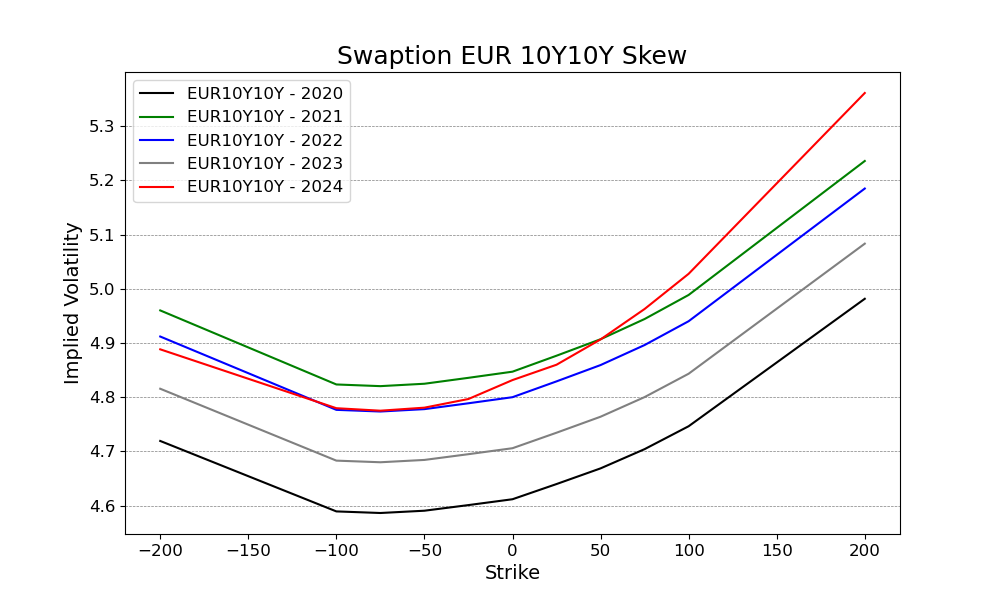
\includegraphics[width=0.9
\textwidth]{/Users/nannaingemannohrt/Desktop/master_thesis/main/plots/10Y10Y_4_smiles.png}
    \caption{EUR swaption 10Y10Y skew over five years. Data source Citi Velocity.}
    \label{fig:rates:smile_5}
\end{figure}

\newpage
\begin{figure}[htbp]
    \centering
    \begin{subfigure}{0.43\textwidth}
        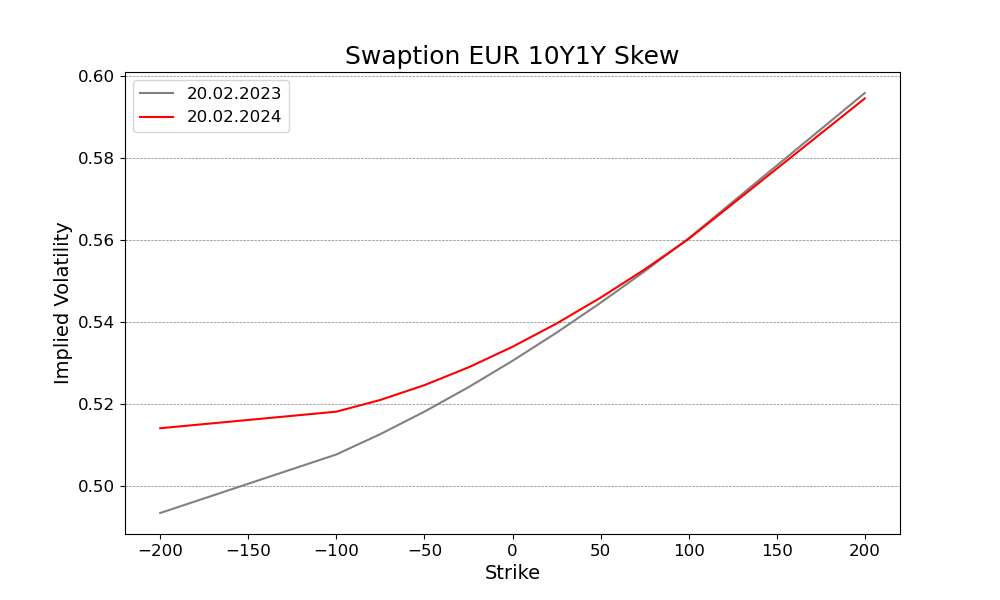
\includegraphics[width=\linewidth]{/Users/nannaingemannohrt/Desktop/master_thesis/main/plots/10Y1Y.png}
        \caption{Volatility Surface EUR swaption 10Y1Y}
        \label{fig:10Y1Y_}
    \end{subfigure}\hfill
    \begin{subfigure}{0.43
        \textwidth}
        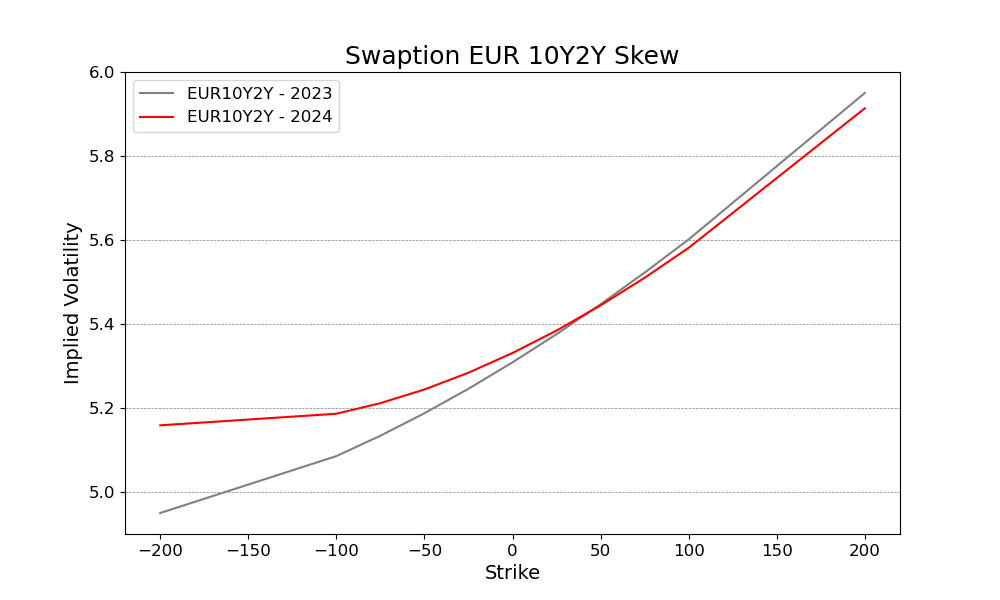
\includegraphics[width=\linewidth]{/Users/nannaingemannohrt/Desktop/master_thesis/main/plots/10Y2Y.png}
        \caption{Volatility Surface EUR swaption 10Y2Y}
        \label{fig:10Y2Y_}
    \end{subfigure}
    \begin{subfigure}{0.43\textwidth}
        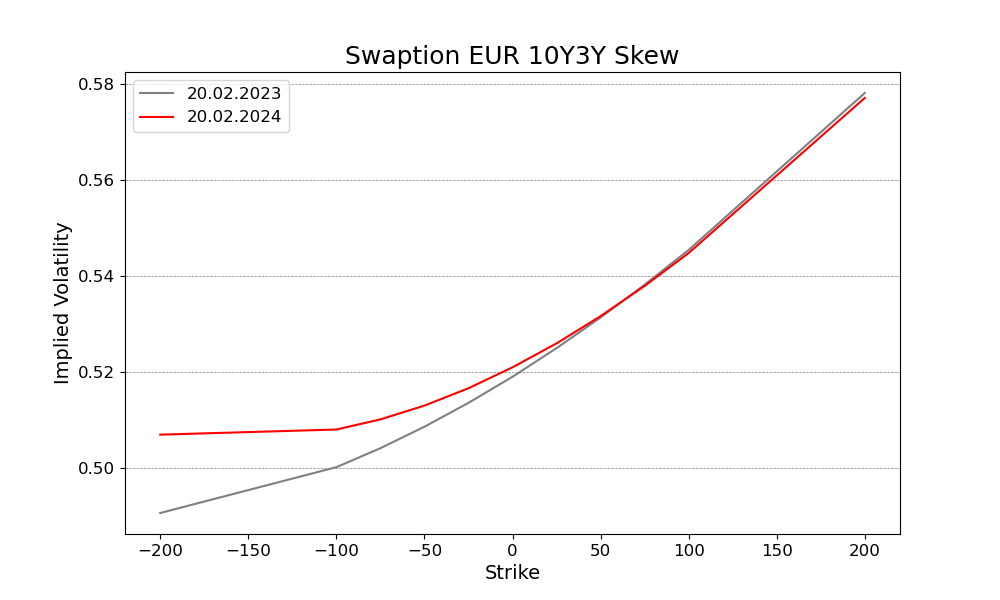
\includegraphics[width=\linewidth]{/Users/nannaingemannohrt/Desktop/master_thesis/main/plots/10Y3Y.png}
        \caption{Volatility Surface EUR swaption 10Y3Y}
        \label{fig:10Y3Y_}
    \end{subfigure}\hfill
    \begin{subfigure}{0.43\textwidth}
        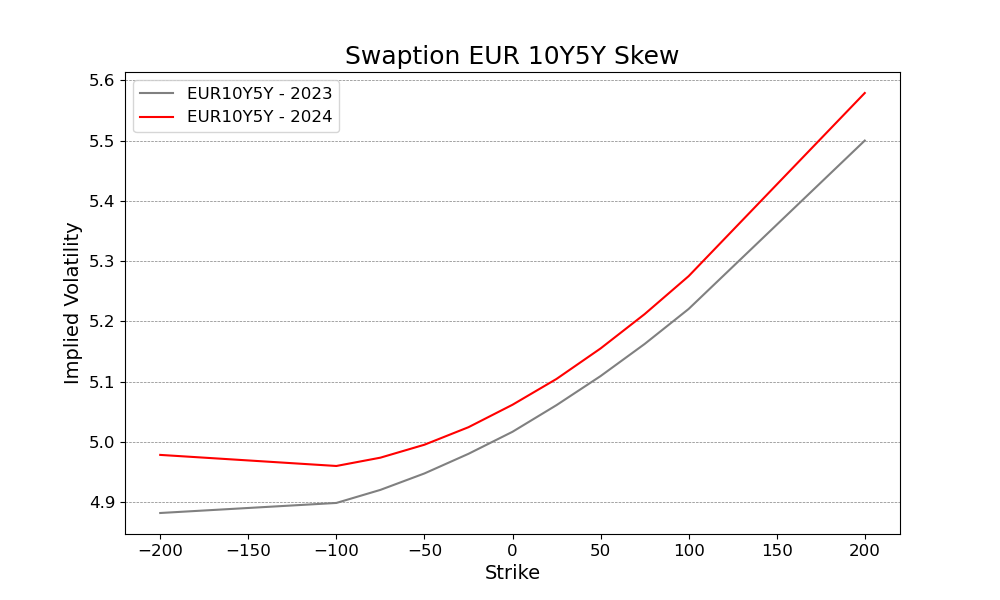
\includegraphics[width=\linewidth]{/Users/nannaingemannohrt/Desktop/master_thesis/main/plots/10Y5Y.png}
        \caption{Volatility Surface EUR swaption 10Y5Y}
        \label{fig:10Y5Y_}
    \end{subfigure}
    \begin{subfigure}{0.43\textwidth}
        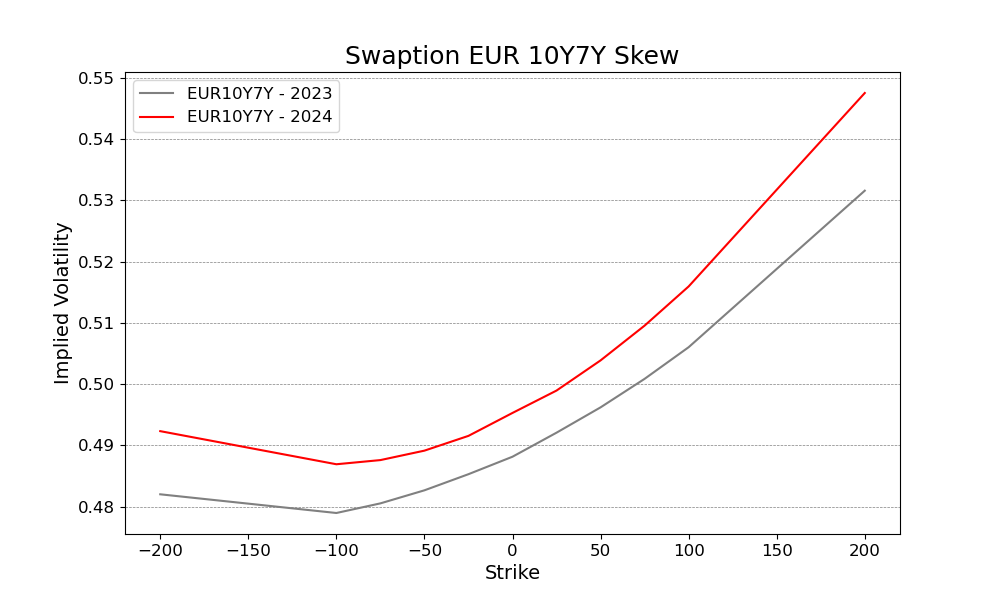
\includegraphics[width=\linewidth]{/Users/nannaingemannohrt/Desktop/master_thesis/main/plots/10Y7Y.png}
        \caption{Volatility Surface EUR swaption 10Y7Y}
        \label{fig:10Y7Y_}
    \end{subfigure}\hfill
    \begin{subfigure}{0.43\textwidth}
        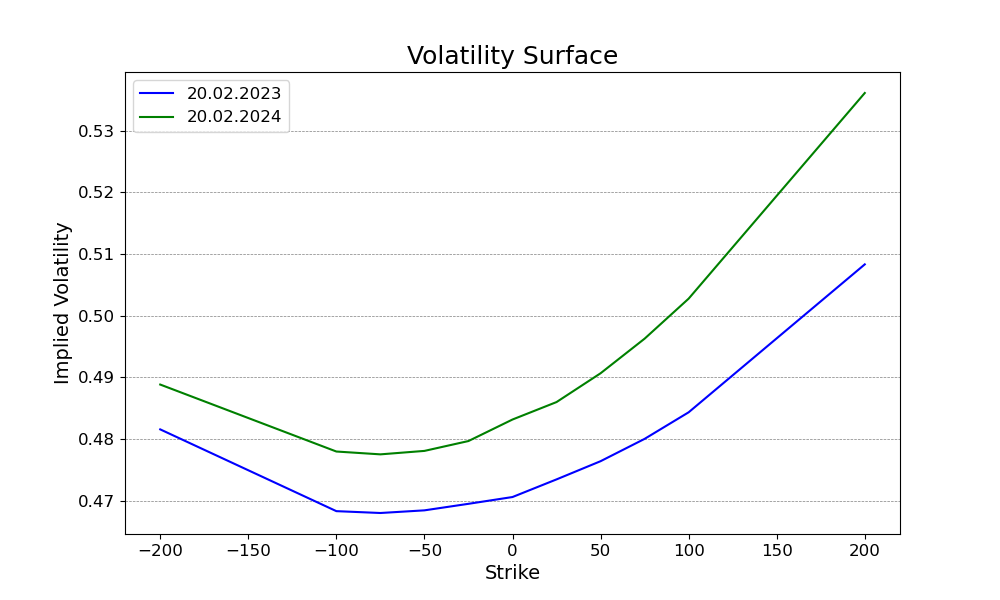
\includegraphics[width=\linewidth]{/Users/nannaingemannohrt/Desktop/master_thesis/main/plots/10Y10Y.png}
        \caption{Volatility Surface EUR swaption 10Y10Y}
        \label{fig:10Y10Y_}
    \end{subfigure}

    \begin{subfigure}{0.43\textwidth}
        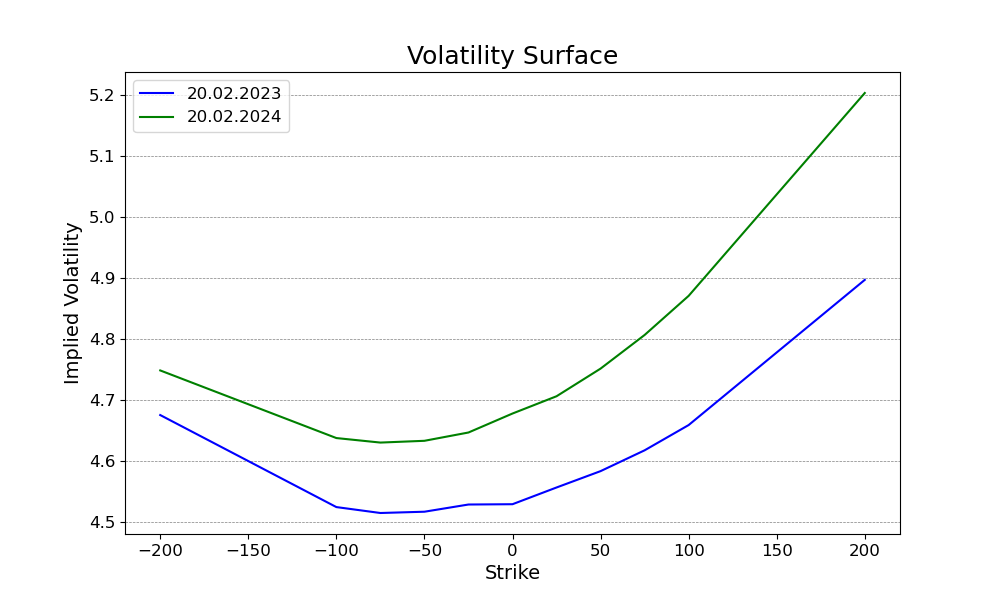
\includegraphics[width=\linewidth]{/Users/nannaingemannohrt/Desktop/master_thesis/main/plots/10Y12Y.png}
        \caption{Volatility Surface EUR swaption 10Y12Y}
        \label{fig:10Y12Y_}
    \end{subfigure}\hfill
    \begin{subfigure}{0.43\textwidth}
        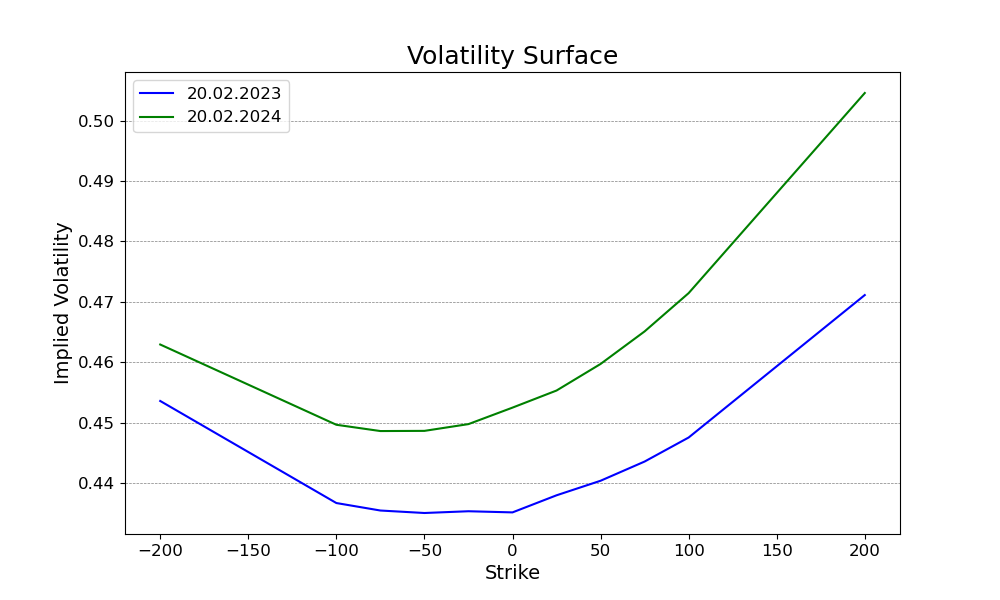
\includegraphics[width=\linewidth]{/Users/nannaingemannohrt/Desktop/master_thesis/main/plots/10Y15Y.png}
        \caption{Volatility Surface EUR swaption 10Y15Y}
        \label{fig:10Y15Y_}
    \end{subfigure}
    \begin{subfigure}{0.43\textwidth}
        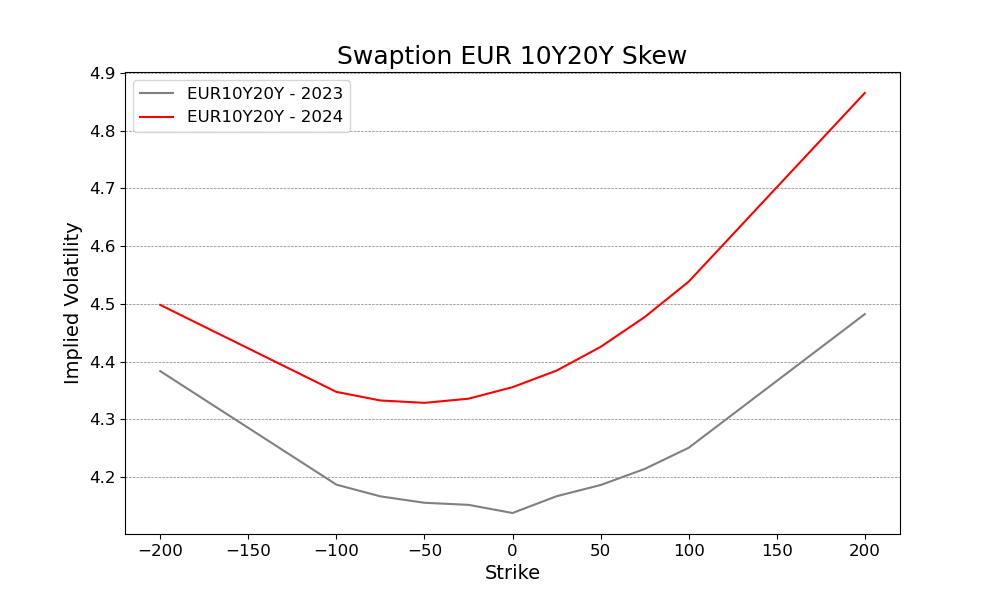
\includegraphics[width=\linewidth]{/Users/nannaingemannohrt/Desktop/master_thesis/main/plots/10Y20Y.png}
        \caption{Volatility Surface EUR swaption 10Y20Y}
        \label{fig:10Y20Y_}
    \end{subfigure}\hfill
    \begin{subfigure}{0.43\textwidth}
        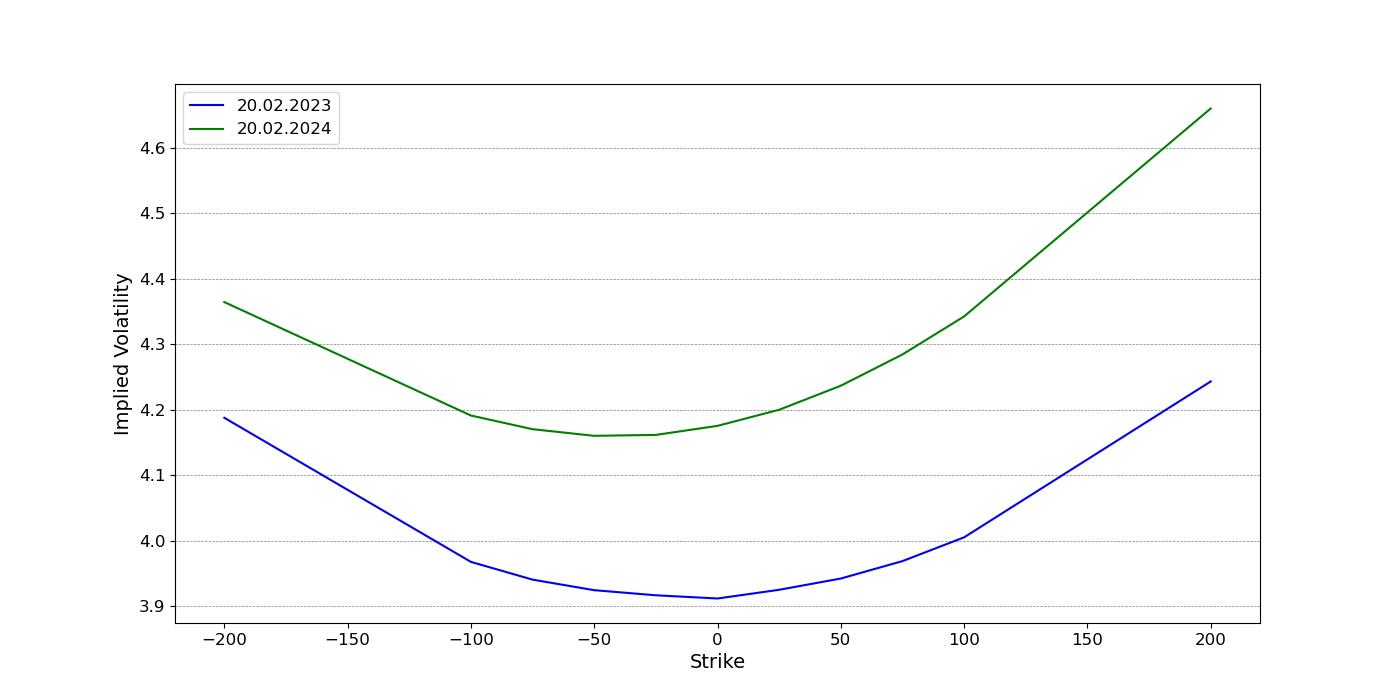
\includegraphics[width=\linewidth]{/Users/nannaingemannohrt/Desktop/master_thesis/main/plots/10Y30Y.png}
        \caption{Volatility Surface EUR swaption 10Y30Y}
        \label{fig:10Y30Y_}
    \end{subfigure}
\end{figure}   